%% LyX 2.3.6.1 created this file.  For more info, see http://www.lyx.org/.
%% Do not edit unless you really know what you are doing.
\documentclass[11pt,oneside,american,czech]{book}
\usepackage[T1]{fontenc}
\usepackage[utf8]{inputenc}
\usepackage[a4paper]{geometry}
\geometry{verbose,tmargin=4cm,bmargin=3cm,lmargin=3cm,rmargin=2cm,headheight=0.8cm,headsep=1cm,footskip=0.5cm}
\pagestyle{headings}
\setcounter{secnumdepth}{3}
\usepackage{url}
\usepackage{amsmath}
\usepackage{amsthm}
\usepackage{amssymb}
\usepackage{graphicx}
\usepackage{setspace}
\usepackage{listings}
\usepackage[dvipsnames]{xcolor}
\usepackage[T1]{fontenc}
\usepackage{lmodern}
\usepackage{pdfpages}
\usepackage{longtable}
\usepackage{multirow}

\definecolor{mygreen}{rgb}{0,0.6,0}
\definecolor{mygray}{rgb}{0.5,0.5,0.5}
\definecolor{mymauve}{rgb}{0.58,0,0.82}
\definecolor{mystring}{rgb}{0.9,0.1,0.2}

\lstset{ 
  backgroundcolor=\color{white},   % choose the background color; you must add \usepackage{color} or \usepackage{xcolor}; should come as last argument
  basicstyle=\scriptsize\fontfamily{cmtt}\selectfont,        % the size of the fonts that are used for the code
  breakatwhitespace=false,         % sets if automatic breaks should only happen at whitespace
  breaklines=true,                 % sets automatic line breaking
  captionpos=t,                    % sets the caption-position to bottom
  commentstyle=\color{mygreen},    % comment style
  stringstyle=\color{mystring},
  deletekeywords={...},            % if you want to delete keywords from the given language
  escapeinside={\%*}{*)},          % if you want to add LaTeX within your code
  extendedchars=true,              % lets you use non-ASCII characters; for 8-bits encodings only, does not work with UTF-8
  firstnumber=1,                   % start line enumeration with line 1000
  frame=single,	                   % adds a frame around the code
  keepspaces=true,                 % keeps spaces in text, useful for keeping indentation of code (possibly needs columns=flexible)
  keywordstyle=\color{blue},       % keyword style
  language=Python,                 % the language of the code
  morekeywords={*,...},            % if you want to add more keywords to the set
  numbers=left,                    % where to put the line-numbers; possible values are (none, left, right)
  numbersep=5pt,                   % how far the line-numbers are from the code
  numberstyle=\tiny\color{mygray}, % the style that is used for the line-numbers
  rulecolor=\color{black},         % if not set, the frame-color may be changed on line-breaks within not-black text (e.g. comments (green here))
  showspaces=false,                % show spaces everywhere adding particular underscores; it overrides 'showstringspaces'
  showstringspaces=false,          % underline spaces within strings only
  showtabs=false,                  % show tabs within strings adding particular underscores
  stepnumber=2,                    % the step between two line-numbers. If it's 1, each line will be numbered
  stringstyle=\color{mymauve},     % string literal style
  tabsize=2,	                   % sets default tabsize to 2 spaces
  title=\lstname                   % show the filename of files included with \lstinputlisting; also try caption instead of title
}

\makeatletter
%%%%%%%%%%%%%%%%%%%%%%%%%%%%%% Textclass specific LaTeX commands.
\newenvironment{lyxlist}[1]
	{\begin{list}{}
		{\settowidth{\labelwidth}{#1}
		 \setlength{\leftmargin}{\labelwidth}
		 \addtolength{\leftmargin}{\labelsep}
		 \renewcommand{\makelabel}[1]{##1\hfil}}}
	{\end{list}}

%%%%%%%%%%%%%%%%%%%%%%%%%%%%%% User specified LaTeX commands.
%% Font setup: please leave the LyX font settings all set to 'default'
%% if you want to use any of these packages:

%% Use Times New Roman font for text and Belleek font for math
%% Please make sure that the 'esint' package is turned off in the
%% 'Math options' page.
\usepackage[varg]{txfonts}

%% Use Utopia text with Fourier-GUTenberg math
%\usepackage{fourier}

%% Bitstream Charter text with Math Design math
%\usepackage[charter]{mathdesign}

%%---------------------------------------------------------------------

%% Make the multiline figure/table captions indent so that the second
%% line "hangs" right below the first one.
%\usepackage[format=hang]{caption}

%% Indent even the first paragraph in each section
\usepackage{indentfirst}

%%---------------------------------------------------------------------

%% Disable page numbers in the TOC. LOF, LOT (TOC automatically
%% adds \thispagestyle{chapter} if not overriden
%\addtocontents{toc}{\protect\thispagestyle{empty}}
%\addtocontents{lof}{\protect\thispagestyle{empty}}
%\addtocontents{lot}{\protect\thispagestyle{empty}}

%% Shifts the top line of the TOC (not the title) 1cm upwards 
%% so that the whole TOC fits on 1 page. Additional page size
%% adjustment is performed at the point where the TOC
%% is inserted.
%\addtocontents{toc}{\protect\vspace{-1cm}}

%%---------------------------------------------------------------------

% completely avoid orphans (first lines of a new paragraph on the bottom of a page)
\clubpenalty=9500

% completely avoid widows (last lines of paragraph on a new page)
\widowpenalty=9500

% disable hyphenation of acronyms
\hyphenation{CDFA HARDI HiPPIES IKEM InterTrack MEGIDDO MIMD MPFA DICOM ASCLEPIOS MedInria}

%%---------------------------------------------------------------------

%% Print out all vectors in bold type instead of printing an arrow above them
\renewcommand{\vec}[1]{\boldsymbol{#1}}

% Replace standard \cite by the parenthetical variant \citep
%\renewcommand{\cite}{\citep}

\makeatother

\usepackage{babel}
\begin{document}
\def\documentdate{2. srpna 2023}

%%\def\documentdate{\today}

\pagestyle{empty}
{\centering

\noindent %
\begin{minipage}[c]{3cm}%
\noindent \begin{center}

\includegraphics[width=3cm,height=3cm,keepaspectratio]{Images/TITLE/cvut}
\par\end{center}%
\end{minipage}%
\begin{minipage}[c]{0.6\linewidth}%
\begin{center}
\textsc{\large{}České vysoké učení technické v Praze}{\large{}}\\
{\large{}Fakulta jaderná a fyzikálně inženýrská}
\par\end{center}%
\end{minipage}%
\begin{minipage}[c]{3cm}%
\noindent \begin{center}

\includegraphics[width=3cm,height=3cm,keepaspectratio]{Images/TITLE/fjfi}
\par\end{center}%
\end{minipage}

\vspace{3cm}

\textbf{\huge{}Moderní metody robustního strojového učení}{\huge\par}

\vspace{1cm}

\selectlanguage{american}%
\textbf{\huge{}Modern methods of robust machine learning}{\huge\par}

\selectlanguage{czech}%
\vspace{2cm}

{\large{}Výzkumný úkol}{\large\par}

}

\vfill{}

\begin{lyxlist}{MMMMMMMMM}
\begin{singlespace}
\item [{Autor:}] \textbf{Bc. Pavel Jakš}
\item [{Vedoucí~práce:}] \textbf{Mgr. Lukáš Adam, Ph.D.}
\item [{Konzultant:}] \textbf{Mgr. Vojtěch Čermák}
\item [{Akademický~rok:}] 2022/2023
\end{singlespace}
\end{lyxlist}
\newpage{}

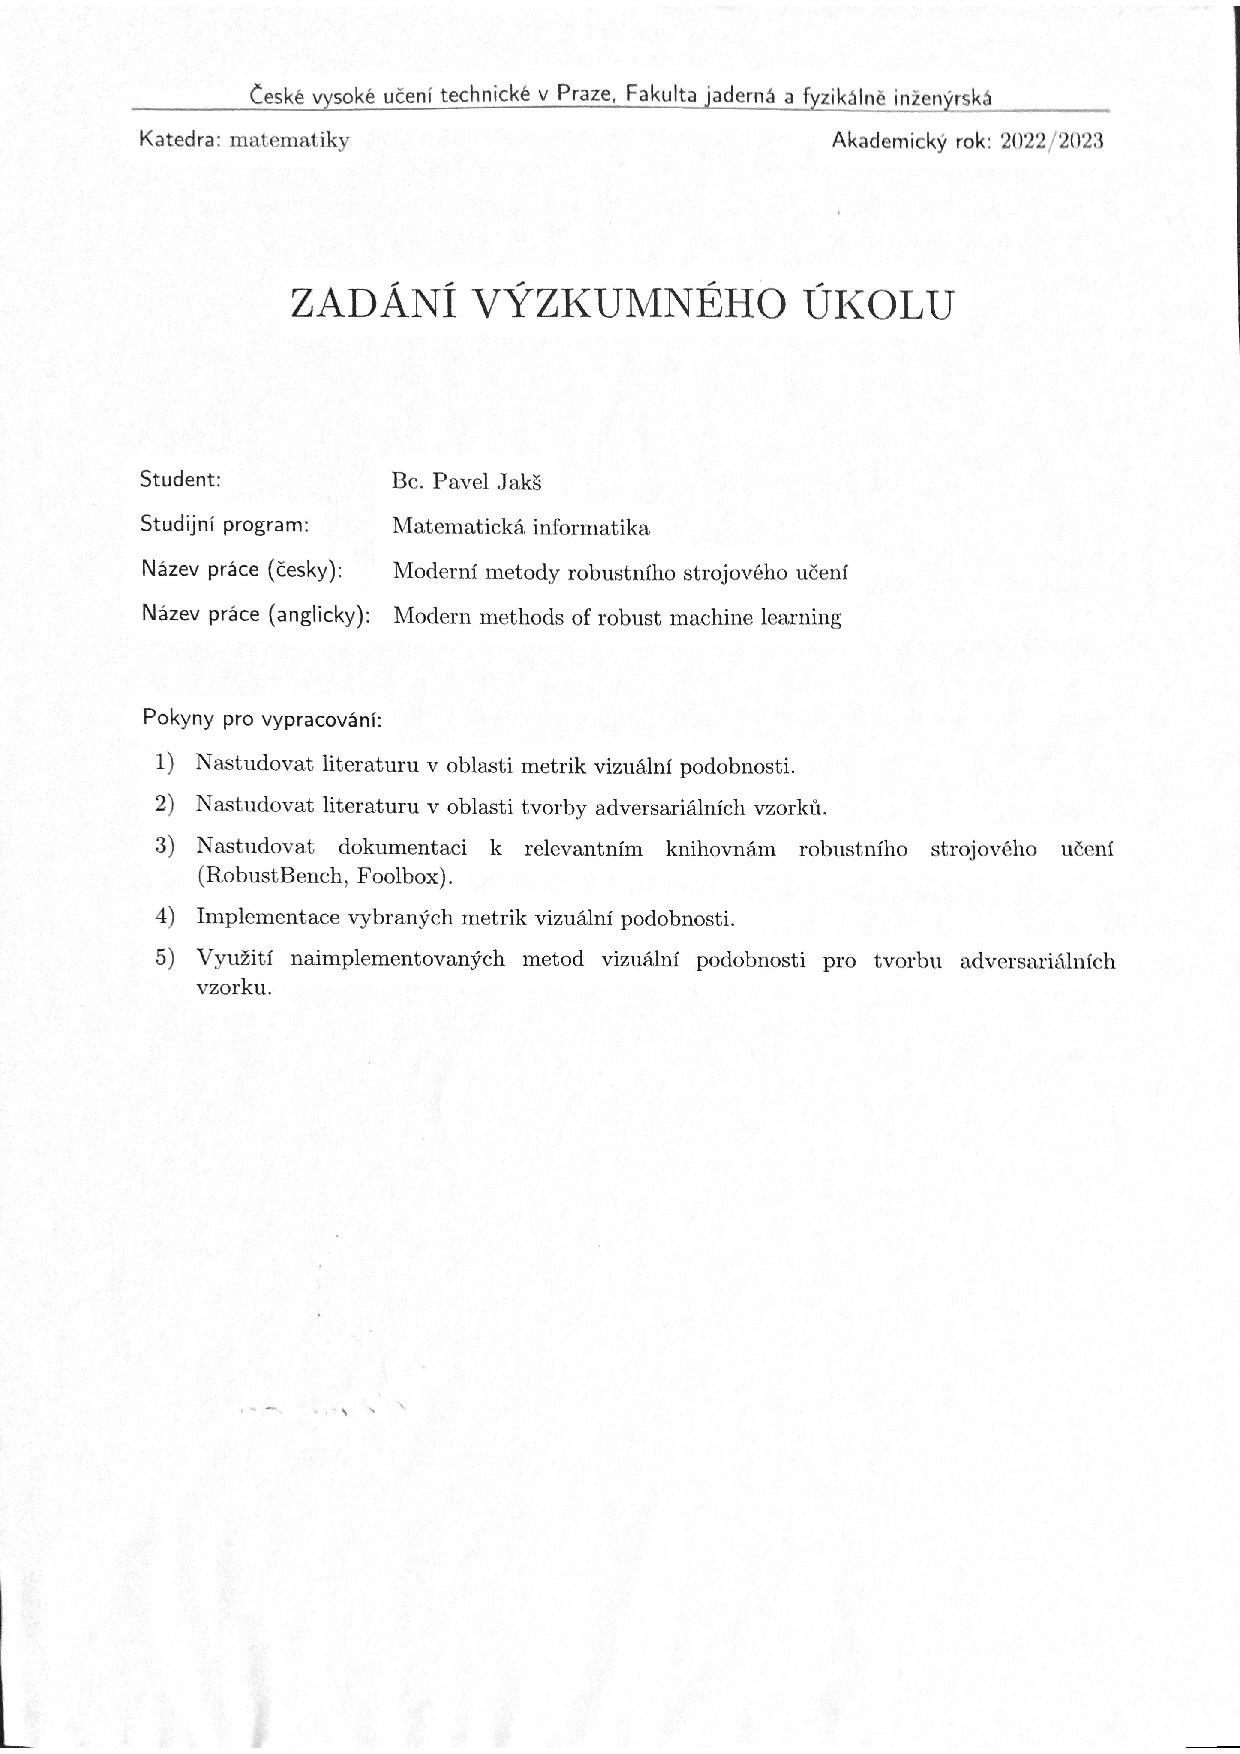
\includepdf{research_project_task.pdf}

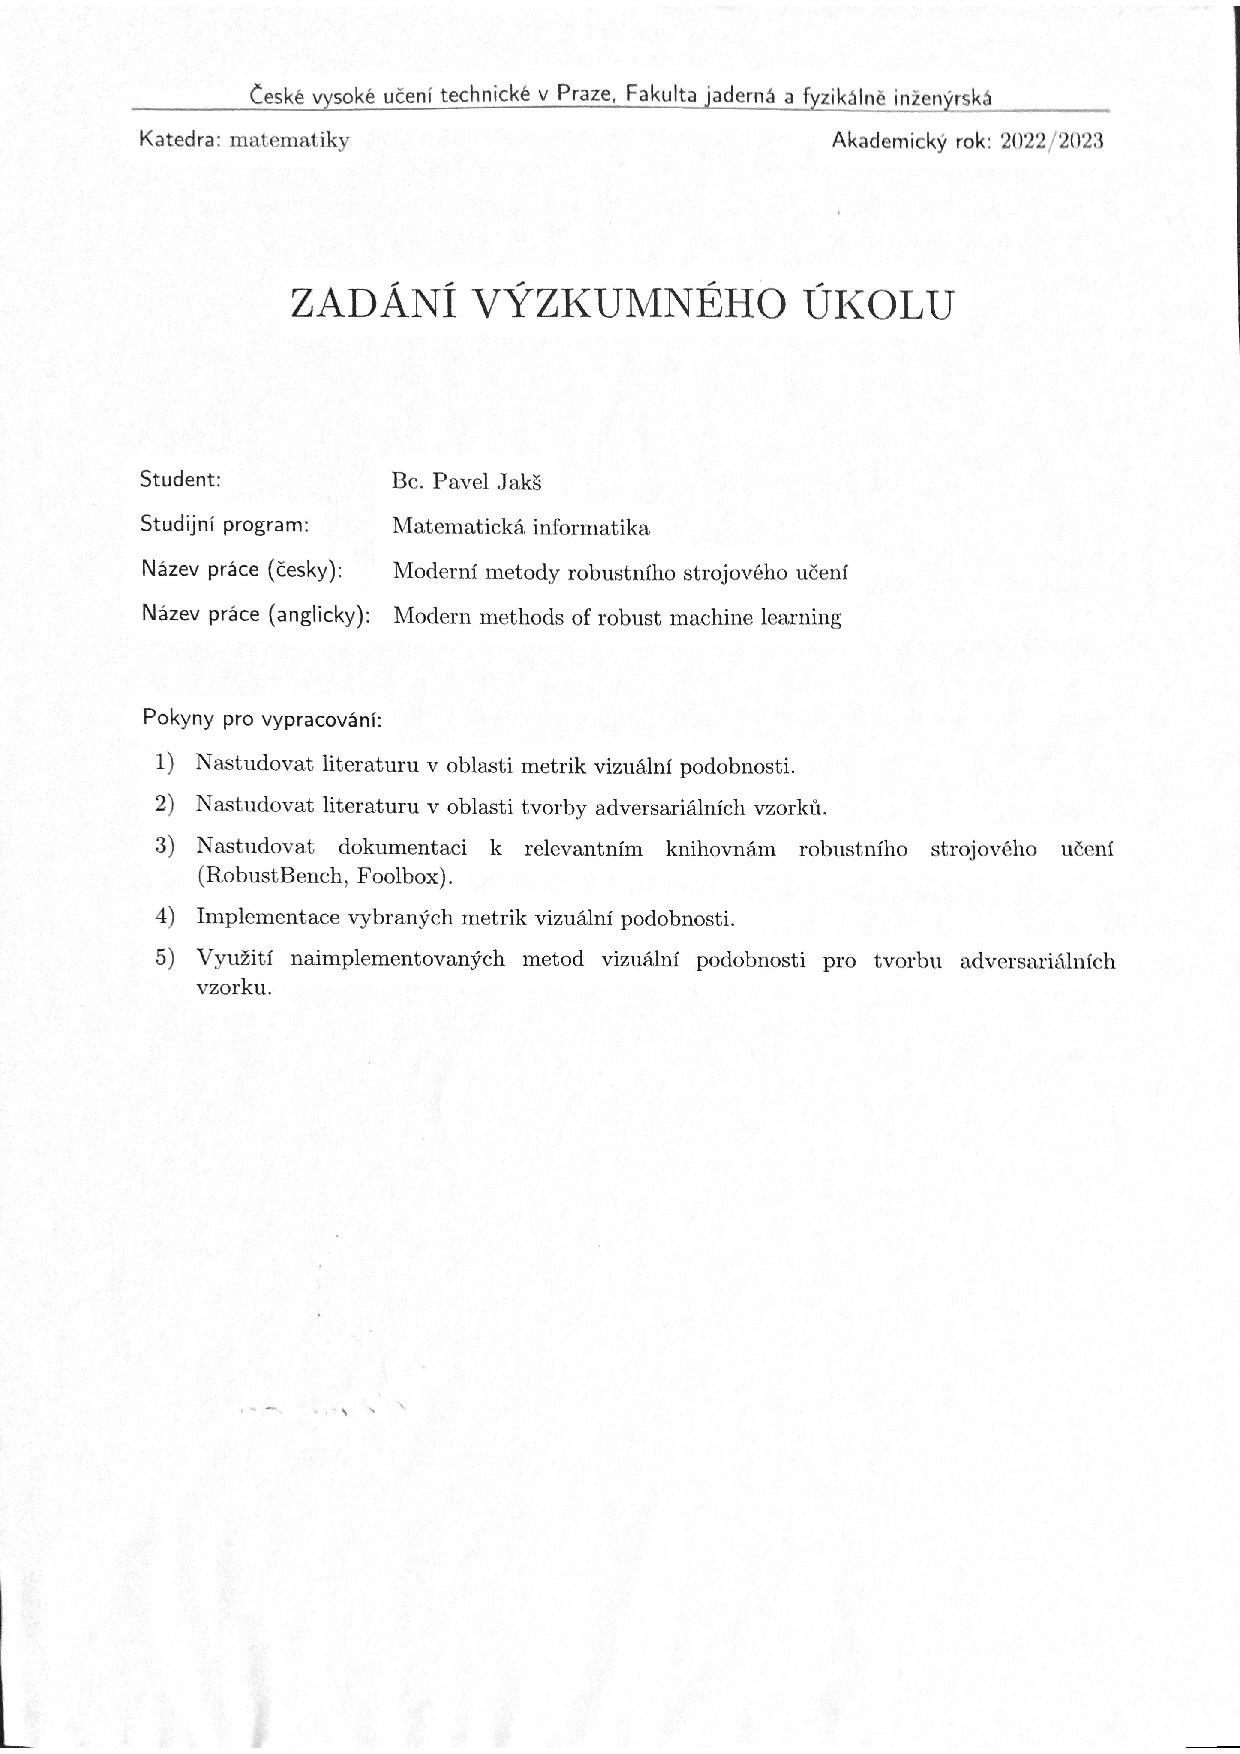
\includepdf[page=2]{research_project_task.pdf}

\newpage{}

\noindent \emph{\Large{}Poděkování:}{\Large\par}

\noindent Chtěl bych zde poděkovat především svému školiteli panu doktoru Adamovi
za pečlivost, ochotu, vstřícnost a odborné i lidské zázemí při vedení
mé diplomové práce. Dále děkuji svému konzultantovi panu magistru Čermákovi
za jeho odborné rady.

\vfill

\noindent \emph{\Large{}Čestné prohlášení:}{\Large\par}

\noindent Prohlašuji, že jsem tuto práci vypracoval samostatně a uvedl
jsem všechnu použitou literaturu.

\bigskip{}

\noindent V Praze dne 21. srpna 2023\hfill{}Bc. Pavel Jakš

\vspace{2cm}

\newpage{}

\begin{onehalfspace}
\noindent \emph{Název práce:}

\noindent \textbf{Moderní metody robustního strojového učení}
\end{onehalfspace}

\bigskip{}

\noindent \emph{Autor:} Bc. Pavel Jakš

\bigskip{}

\noindent \emph{Obor:} Matematická informatika\bigskip{}

\bigskip{}

\noindent \emph{Druh práce:} Výzkumný úkol

\bigskip{}

\noindent \emph{Vedoucí práce:} Mgr. Lukáš Adam, Ph.D.,
Katedra počítačů,
Fakulta elektrotechnická,
České vysoké učení technické v Praze,
Karlovo náměstí 13, 121 35 Praha 2.

\bigskip{}

\noindent \emph{Konzultant:} Mgr. Vojtěch Čermák,
Katedra počítačů,
Fakulta elektrotechnická,
České vysoké učení technické v Praze,
Karlovo náměstí 13, 121 35 Praha 2.

\bigskip{}

\noindent \emph{Abstrakt:} Abstrakt max. na 10 řádků. Abstrakt max.
na 10 řádků. Abstrakt max. na 10 řádků. Abstrakt max. na 10 řádků.
Abstrakt max. na 10 řádků. Abstrakt max. na 10 řádků. Abstrakt max.
na 10 řádků. Abstrakt max. na 10 řádků. Abstrakt max. na 10 řádků.
Abstrakt max. na 10 řádků. Abstrakt max. na 10 řádků. Abstrakt max.
na 10 řádků. Abstrakt max. na 10 řádků. Abstrakt max. na 10 řádků.
Abstrakt max. na 10 řádků. Abstrakt max. na 10 řádků. Abstrakt max.
na 10 řádků. Abstrakt max. na 10 řádků. Abstrakt max. na 10 řádků.
Abstrakt max. na 10 řádků. Abstrakt max. na 10 řádků. Abstrakt max.
na 10 řádků. Abstrakt max. na 10 řádků. Abstrakt max. na 10 řádků.
Abstrakt max. na 10 řádků. Abstrakt max. na 10 řádků. Abstrakt max.
na 10 řádků. Abstrakt max. na 10 řádků. Abstrakt max. na 10 řádků. 

\bigskip{}

\noindent \emph{Klíčová slova:} klíčová slova (nebo výrazy) seřazená
podle abecedy a oddělená čárkou

\vfill{}
~

\selectlanguage{american}%
\begin{onehalfspace}
\noindent \emph{Title:}

\noindent \textbf{Modern methods of robust machine learning}
\end{onehalfspace}

\bigskip{}

\noindent \emph{Author:} Bc. Pavel Jakš

\bigskip{}

\noindent \emph{Abstract:} Max. 10 lines of English abstract text.
Max. 10 lines of English abstract text. Max. 10 lines of English abstract
text. Max. 10 lines of English abstract text. Max. 10 lines of English
abstract text. Max. 10 lines of English abstract text. Max. 10 lines
of English abstract text. Max. 10 lines of English abstract text.
Max. 10 lines of English abstract text. Max. 10 lines of English abstract
text. Max. 10 lines of English abstract text. Max. 10 lines of English
abstract text. Max. 10 lines of English abstract text. Max. 10 lines
of English abstract text. Max. 10 lines of English abstract text.
Max. 10 lines of English abstract text. Max. 10 lines of English abstract
text. Max. 10 lines of English abstract text. Max. 10 lines of English
abstract text. Max. 10 lines of English abstract text. Max. 10 lines
of English abstract text. Max. 10 lines of English abstract text.
Max. 10 lines of English abstract text. Max. 10 lines of English abstract
text. Max. 10 lines of English abstract text.

\bigskip{}

\noindent \emph{Key words:} keywords in alphabetical order separated
by commas

\selectlanguage{czech}%
\newpage{}

\pagestyle{plain}

\tableofcontents{}

\newpage{}

\chapter*{Úvod}

\addcontentsline{toc}{chapter}{Úvod}

Text úvodu....

\chapter{Metriky vizuální podobnosti}

Pod pojmem metrika na prostoru $X$ si každý matematik představí zobrazení $\rho : X \times X \rightarrow [0, + \infty)$
splňující
\begin{enumerate}
    \item $\rho(x, y) = 0 \iff x = y \quad \forall x, y \in X$,
    \item $\rho(x, y) = \rho(y, x) \quad \forall x, y \in X$,
    \item $\rho(x, z) \leq \rho(x, y) + \rho(y, z) \quad \forall x, y, z \in X$.
\end{enumerate}

Taková metrika může být na lineárním prostoru $V$ nad číselným tělesem (pro naše účely zůstaňme nad $\mathbb{R}$)
snadno zadána pomocí normy,
která je buď indukována skalárním součinem v případě pre-Hilbertových prostorů,
nebo dána vlastnostmi, že se jedná o zobrazení $\|.\| : V \rightarrow [0, + \infty)$
a splňuje:
\begin{enumerate}
    \item $\|x\| = 0 \iff x = 0 \quad \forall x \in V$,
    \item $\|\alpha x\| = |\alpha| \cdot \|x\| \quad \forall \alpha \in \mathbb{R}, \forall x \in V$,
    \item $\|x + y\| \leq \|x\| + \|y\| \quad \forall x, y \in V$.
\end{enumerate}
Metriku potom získáme z normy následující konstrukcí:
\begin{equation*}
    \rho (x, y) = \| x - y \|,
\end{equation*}
tedy vzdálenost dvou vektorů je dána normou rozdílu vektorů.
Snadno lze nahlédnout, že takto zadané zobrazení je metrika.
S metrikami, které jsou tzv. indukované normami dle předchozího se setkáme.


\section{Metriky indukované $l_p$ normami}

Vzhledem k tomu, že obrázky, které jsou středem naší pozornosti,
lze reprezentovat jako tenzory standardně o rozměrech $C \times W \times H$,
kde $C$ značí počet kanálů (nejčastěji kanály po řadě pro červenou, zelenou a modrou barvu),
$W$ označuje šířku a $H$ výšku, tak lze na tyto tenzory vpustit $L^p$ normy.
Pro $p \in [1, + \infty)$ je $L^p$ norma z $f \in L_p(X, \mu )$
definována vztahem:
\begin{equation*}
    \|f\|_p = \left(\int_X |f|^p \mathrm{d} \mu \right)^{\frac{1}{p}}.
\end{equation*}

Pro naše obrázky lze za $X$ vzít $\{1, ... C\} \times \{1, ..., W\} \times \{1, ..., H\}$ a za $\mu$ \emph{počítací míru}.
Potom naše $L^p$ norma přejde v $l_p$ normu, která má pro naše obrázky, tedy tenzory $x \in \mathbb{R}^{C \times W \times H}$, tvar:
\begin{equation}
    \|x\|_p = \left( \sum_{i=1}^{C} \sum_{j=1}^{W} \sum_{k=1}^{H} |x_{i, j, k}|^p \right)^{\frac{1}{p}}.
\end{equation}

Trochu mimo stojí $l_{\infty}$ norma, která má tvar pro tenzor $x \in \mathbb{R}^{C \times W \times H}$:
\begin{equation}
    \|x\|_\infty = \max_{i \in \{1, ..., C\}} \max_{j \in \{1, ..., W\}} \max_{k \in \{1, ..., H\}} |x_{i, j, k}|.
\end{equation}

A úplně mimo stojí $L_0$ norma, která svou povahou \emph{není} norma ve smyslu výše uvedené definice,
ale pro účely porovnávání obrázků se používá rozdíl obrázků v této pseudo-normě, proto ji zde zmiňuji:
\begin{equation}
    \|x\|_0 = |\{x_{i, j, k} \neq 0\}|.
\end{equation}

\section{MSE a RMSE}

Vzdálenosti, které mají blízko k metrikám indukovaným $l_2$ normou, jsou \emph{MSE} (z anglického \emph{Mean Squared Error})
a \emph{RMSE} (z anglického \emph{Root Mean Squared Error}).
Pro tenzory $x, \tilde{x} \in \mathbb{R}^{C \times W \times H}$ mají definici:
\begin{align}
    \operatorname{MSE}(x, \tilde{x}) &= \frac{1}{C W H} \sum_{i=1}^C \sum_{j=1}^W \sum_{k=1}^H | x_{i, j, k} - \tilde{x}_{i, j, k} |^2 \\
    \operatorname{RMSE}(x, \tilde{x}) &= \left(\frac{1}{C W H} \sum_{i=1}^C \sum_{j=1}^W \sum_{k=1}^H | x_{i, j, k} - \tilde{x}_{i, j, k} |^2 \right)^{\frac{1}{2}}
\end{align}

\section{Peak signal-to-noise ratio}

Vzdálenost označená zkratkou \emph{PSNR} z anglického \emph{peak signal-to-noise ratio}
vyjadřuje vztah mezi obrázkem $x \in \mathbb{R}^{C \times W \times H}$
a jeho pokažením $\tilde{x} \in \mathbb{R}^{C \times W \times H}$ za přidání šumu.
Definice je následující:
\begin{align}
    \operatorname{PSNR}(x, \tilde{x}) &= 10 \cdot \operatorname{log}_{10} \left( \frac{l^2}{\operatorname{MSE}(x, \tilde{x})} \right), \\
    &= 20 \cdot \operatorname{log}_{10} \left( \frac{l}{\operatorname{RMSE}(x, \tilde{x})} \right),
\end{align}
kde $l$ je dynamický rozsah obrázků, tedy rozdíl mezi maximální možnou hodnotou pixelů a minimální možnou hodnotou pixelů.
% Jak je vidět, prohození $x$ a $\tilde{x}$ povede ke změně hodnoty $\operatorname{PSNR}$, tato vzdálenost tedy není metrická.
Jedná se tedy o transformaci metriky \emph{MSE}.
Samotná hodnota PSNR ovšem není metrická vzdálenost.
Vždyť budou-li se obrázky $x$ a $\tilde{x}$ blížit k sobě, hodnota $\operatorname{PSNR}(x, \tilde{x})$ poroste do nekonečna.

\section{Wassersteinova vzdálenost}

Buď $(M, d)$ metrický prostor, který je zároveň \emph{Radonův}. Zvolme $p \in [1, + \infty)$.
Potom máme \emph{Wassersteinovu $p$-vzdálenost} mezi dvěma pravděpodobnostními mírami $\mu$ a $\nu$ na $M$,
které mají konečné $p$-té momenty,
jako:
\begin{equation}
    W_p (\mu, \nu) = \left( \inf_{\gamma \in \Gamma(\mu, \nu)} \mathbb{E}_{(x, y) \sim \gamma} d(x, y)^p \right)^{\frac{1}{p}},
\end{equation}
kde $\Gamma(\mu, \nu)$ je množina všech sdružených pravděpodobnostních měr na $M \times M$,
které mají po řadě $\mu$ a $\nu$ za marginální pravděpodobnostní míry \cite{vaserstejn}.

Jak to souvisí s obrázky?
Přes dopravní problém.
Pod pravděpodobnostní distribucí $\mu$ či $\nu$ na $X$ si lze představit rozložení jakési hmoty
o celkové hmotnosti $1$.
Sdružená rozdělení $\gamma \in \Gamma(\mu, \nu)$ potom odpovídají transportnímu plánu,
kde $\gamma(x, y) \operatorname{d}x \operatorname{d}y$
vyjadřuje, kolik hmoty se přesune z $x$ do $y$.
Tomu lze přiřadit nějakou cenu $c$,
totiž kolik stojí přesun jednotkové hmoty z $x$ do $y$: $c(x, y)$.
V případě \emph{Wassersteinovy vzdálenosti}
za cenu dosadíme $c(x, y) = d(x, y)^p$,
tedy $p$-tou mocninu vzdálenosti mezi $x$ a $y$.
Potom cena celkového dopravního problému s transportním plánem $\gamma$ bude:
\begin{align}
    c_\gamma &= \int c(x, y) \gamma(x, y) \operatorname{d}x \operatorname{d}y \\
    &= \int c(x, y) \operatorname{d} \gamma(x, y)
\end{align}
a optimální cena bude:
\begin{equation}
    c = \inf_{\gamma \in \Gamma(\mu, \nu)} c_\gamma.
\end{equation}
Po dosazení:
\begin{align}
    c &= \inf_{\gamma \in \Gamma(\mu, \nu)} \int c(x, y) \operatorname{d} \gamma(x, y) \\
    &= \inf_{\gamma \in \Gamma(\mu, \nu)} \int c(x, y) \gamma(x, y) \operatorname{d}x \operatorname{d}y \\
    &= \inf_{\gamma \in \Gamma(\mu, \nu)} \mathbb{E}_{(x, y) \sim \gamma} c(x, y) \\
    &= \inf_{\gamma \in \Gamma(\mu, \nu)} \mathbb{E}_{(x, y) \sim \gamma} d(x, y)^p \\
    &= W_p (\mu, \nu)^p
\end{align}
Dostáváme tedy interpretaci, že $p$-tá mocnina \emph{Wassersteinovy vzdálenosti}
odpovídá ceně dopravního problému.

Pro obrázky má tato konstrukce následující uplatnění:
Obrázky je třeba chápat jako diskrétní pravděpodobnostní rozdělení,
proto je třeba je normalizovat,
aby součet prvků tenzoru obrázku byl roven $1$.
Pak střední hodnota v definici Wassersteinovy vzdálenosti přejde ve váženou sumu cen,
tedy $p$-tých mocnin vzdáleností mezi jednotlivými pixely.

Jak je to barevnými obrázky, tedy s obrázku, které mají více než jeden kanál?
Zde lze uplatnit následující dva přístupy:
\begin{enumerate}
    \item Normovat celý obrázek na jedničku, tedy všechny kanály dohromady, a tím pádem i definovat vzdálenost mezi jednotlivými kanály,
    \item Normovat každý kanál zvlášť na jedničku, počítat Wassersteinovu metriku pro každý kanál zvlášť
    a následně vybrat nějakou statistiku výsledných vzdáleností, např. průměr.
\end{enumerate}

\section{Structural similarity index measure}

Zkratka \emph{SSIM} pochází z anglického \emph{structural similarity index measure}.
Tato metrika se při výpočtu indexu dvou obrázků $x$ a $\tilde{x}$ dívá na podokna,
ze kterých vybere jisté statistiky a z nich vytvoří index pro daná podokna obrázků.
Potom se jako celkový index bere průměr přes tato okna.
Uveďme vzorce pro výpočet indexu SSIM pro případ, že máme jediné okno, které splývá s obrázkem,
které pro jednoduchost zvolme jednokanálové, tedy černobílé.
Označme $N = W \times H$ počet pixelů v obrázku a indexujme prvky matice obrázku jediným číslem.
Potom definujeme pro obrázky $x$ a $\tilde{x}$ následující:
\begin{align*}
    \mu_x &= \frac{1}{N} \sum_{i = 1}^N x_i, \\
    \mu_{\tilde{x}} &= \frac{1}{N} \sum_{i = 1}^N \tilde{x}_i, \\
    \sigma_x^2 &= \frac{1}{N - 1} \sum_{i = 1}^N (x_i - \mu_x)^2, \\
    \sigma_{\tilde{x}}^2 &= \frac{1}{N - 1} \sum_{i = 1}^N (\tilde{x}_i - \mu_{\tilde{x}})^2, \\
    \sigma_{x \tilde{x}} &= \frac{1}{N - 1} \sum_{i = 1}^N (x_i - \mu_x)(\tilde{x}_i - \mu_{\tilde{x}}).
\end{align*}
Potom:
% Pod zkratkou \emph{SSIM} (\emph{Structural Similarity Index Measure})
% se rozumí následující vzdálenost:
\begin{equation}
    \operatorname{SSIM}(x, \tilde{x}) = \frac{(2 \mu_x \mu_{\tilde{x}} + C_1)(2 \sigma_{x \tilde{x}} + C_2)}{(\mu_x^2 + \mu_{\tilde{x}}^2 + C_1)(\sigma_x^2 + \sigma_{\tilde{x}}^2 + C_2)},
\end{equation}
% kde $\mu$ je průměr hodnot pixelů $x$, resp. $\tilde{x}$,
% $\sigma_{x \tilde{x}}$ je nestranný odhad kovariance mezi $x$ a $\tilde{x}$,
% $\sigma^2$ je nestranný odhad rozptylu $x$, resp. $\tilde{x}$
kde $C_1, C_2$ jsou konstanty pro stabilitu dělení volené kvadraticky úměrně dynamickému rozsahu.
% Máme-li dva obrázky, tak za $x$ a $\tilde{x}$ do vzorce pro $\operatorname{SSIM}$ se standardně volí jakási okna obrázků.
% To znamená, že za celkovou vzdálenost mezi dvěma obrázky volíme průměr přes všechna okna předem zvolené velikosti.
Můžeme si povšimnout, že $\operatorname{SSIM}(x, \tilde{x})$ není metrická vzdálenost.
Budou-li obrázky stejné, nevyjde $0$, nýbrž $1$.
Může se také stát, že SSIM vrátí zápornou hodnotu, která může vzniknout členem $\sigma_{x \tilde{x}}$.
Jak volíme celkový SSIM pro barevné obrázky?
Jako průměr přes kanály.



\chapter{Implementace metrik vizuální podobnosti}

V minulé kapitole jsme viděli přehled metod, jak přistoupit k porovnávání dvou různých obrázků.
Předvedli jsme, jak vyčíslit rozdíl mezi dvěma obrázky.
Ne vždy se ovšem jedná o metriku vesmyslu matematickém,
což pro tvorbu adversariálních vzorků je záhodno,
a ne vždy lze takovouto vzdálenost přímočaře spočíst.
Proto uveďme, je-li to nutné, příslušné úkroky stranou, které nám umožní hledat adversariální vzorky,
a to pokud možno v krátkém čase.
Samotnou výslednou implementaci v podobě kódu v jazyce python lze nalézt v příloze v části týkající se souboru \emph{metrics.py}.

\section{Metriky založené na $l_p$ normách}

Implementovat klasické $l_p$ normy je snadné, a tedy i metriky jimi indukované.
MSE a RMSE jsou též snadné na implementaci.
Vlastně i PSNR.
Metriku vizuální podobnosti PSNR je třeba ovšem ošetřit,
neboť, jak již bylo poznamenáno,
budou-li se obrázky $x$ a $\tilde{x}$ blížit k sobě,
hodnota $\operatorname{PSNR}(x, \tilde{x})$ poroste do nekonečna.
Proto zkusme vzít konstrukci, kde prohodíme roli dynamického rozsahu $l$ (peak signal) s rolí šumu (noise),
dostaneme tedy, co lze nazvat noise to peak signal ratio (NPSR):
\begin{align}
    \operatorname{NPSR}(x, \tilde{x}) &= 20 \cdot \operatorname{log}_{10} \left( \frac{\operatorname{RMSE}(x, \tilde{x})}{l} \right), \\
    &= - \operatorname{PSNR}(x, \tilde{x}).
\end{align}
Při dvou obrázcích blížících se k sobě bude tedy NPSR klesat, a to neomezeně.


\section{Modifikace Wassersteinovy vzdálenosti}

Abychom mohli s Wassersteinovou metrikou nakládat například v počítači, je nutné tuto metriku spočíst.
Podíváme-li se do definice, znamená to vyřešit optimalizační problém.
Byť bychom se omezili hledání vzdáleností dvou vektorů o~rozměru $q$,
měli bychom problém s časovou složitostí nejlépe $\mathcal{O}(q^3 \operatorname{log} q)$ \cite{wass_computation}.
A~to je hodně.
Proto se podívejme, jak Wassersteinovu vzdálenost spočíst rychleji, byť za ztráty přesnosti.

Omezme se na prostory konečné dimenze. Potom mějme za úkol spočíst Wassersteinovu  (zvolme $p = 1$) vzdálenost vektorů
$\mu, \nu \in \mathbb{R}^q, \mu ^ T 1_q = \nu ^ T 1_q = 1$, kde $1_q$ je vektor rozměru $q$ složen pouze z jedniček.
Potom $\mu, \nu$ lze chápat jako diskrétní pravděpodobnostní rozdělení.
Označme jako $U(\mu, \nu)$ množinu všech matic $P \in \mathbb{R}^{q \times q}, P_{i,j} \geq 0$
takových, že $P 1_q = \mu$ a $P^T 1_q = \nu$.
Jako matici $C$ označme zadanou matici cen, která splňuje, že reprezentuje metriku.
To znamená, že $C_{i, j} \geq 0$, $C_{i, j} = 0 \iff i = j$, $C_{i, j} = C_{j, i}$ a $C_{i, k} \leq C_{i, j} + C_{j, k}$.
Potom lze napsat:
\begin{equation}
    W (\mu, \nu) \equiv W_1 (\mu, \nu) = \min_{P \in U(\mu, \nu)} \langle P, C \rangle,
\end{equation}
kde $\langle P, C \rangle = \sum_{i, j = 1}^q P_{i, j} C_{i, j}$.

Přejděme nyní od Wassersteinovy metriky k tzv. duální Sinkhornově metrice.
Ta je pro pevně zvolené $\lambda > 0$ definována následovně:
\begin{align}
    W^\lambda (\mu, \nu) &= \langle P^\lambda, C \rangle, \\
    kde \; P^\lambda &= \operatornamewithlimits{argmin}_{P \in U(\mu, \nu)} \langle P, C \rangle - \frac{1}{\lambda} H(P),
\end{align}
kde $H(P)$ je entropie pravděpodobnostního rozdělení $P$, tedy 
\begin{equation*}
    H(P) = - \sum_{i, j = 1}^q P_{i, j} \operatorname{log}(P_{i, j}).
\end{equation*}
Jedná se tedy o regularizovaný dopravní problém.
Tato úprava Wassersteinovy metriky je, jak se přesvědčíme, mnohem lépe vyčíslitelná.
Nejdříve se ovšem podívejme na intuici za touto úpravou.

Začněme s mírnou úpravou původního optimalizačního problému definujícího Wassersteinovu vzdálenost:
Pro $\alpha > 0$ definujme jakési $\alpha$ okolí rozdělení $\mu \nu^T$
(sdružené pravděpodobnostní rozdělení s marginálními $\mu$ a $\nu$, kde $\mu$ a $\nu$ jsou nezávislá rozdělení) ve smyslu
\emph{Kullback-Leiblerovy divergence}
\begin{equation}
    U_{\alpha} (\mu, \nu) = \{P \in U(\mu, \nu) | KL(P \| \mu \nu^T) \leq \alpha\}.
\end{equation}
Připomeňme definici Kullback-Leiblerovy divergence:
\begin{equation*}
    KL(\tilde{P} \| \hat{P}) = \sum_{i, j = 1}^q P_{i, j} \operatorname{log} \frac{P_{i, j}}{ Q_{i, j}}.
\end{equation*}
Pro dané $P \in U(\mu, \nu)$ lze na kvantitu $KL(P \| \mu \nu^T)$ nahlédnout jako na informaci mezi veličinami s rozděleními $\mu$ a $\nu$.
Tedy $U_\alpha (\mu, \nu)$ vybírá ta rozdělení, která nesou malou vzájemnou informaci mezi $\mu$ a $\nu$ (ve smyslu menší než $\alpha$).
Dle \cite{wass_computation} lze tuto úpravu ospravedlnit pomocí \emph{principu maximální entropie}.

Potom lze definovat následující Sinkhornovu metriku:
\begin{equation}
    W^\alpha (\mu, \nu) = \min_{P \in U_\alpha (\mu, \nu)} \langle P, M \rangle.
\end{equation}
Jaký je vztah mezi Sinkhornovou metrikou $W^\alpha$ a duální Sinkhornovou metrikou $W^\lambda$?
Přes téma duality matematického programování.
Zatímco ve $W^\alpha$ figuruje parametr $\alpha$ v omezení definičního oboru, kde optimalizujeme,
tak ve $W^\lambda$ figuruje parametr $\lambda$ jako Lagrangeův multiplikátor příslušné vazby.

% Snadno lze nahlédnout na ekvivalentní definici $U_{\alpha} (\mu, \nu)$:
% \begin{equation}
%     U_{\alpha} (\mu, \nu) = \{P \in U(\mu, \nu) | H(P) \geq H(\mu) + H(\nu) - \alpha\}.    
% \end{equation}
% Tedy chtěli bychom řešit optimalizační problém Sinkhornovy metriky.
% Lagrangeova funkce by vypadala následovně:
% \begin{equation}
%     \mathcal{L}(P, \lambda) = \langle P, M \rangle - \frac{1}{\lambda} ()
% \end{equation}

Článek \cite{wass_computation} poskytuje též nahlédnutí na fakt, že $W^\lambda$ a $W^\alpha$ jsou skutečně metriky.

Tento úkrok stranou pomocí entropické regularizace původního problému lineárního programování,
jehož vyřešení je nutné pro výpočet Wassersteinovy vzdálenosti, poskytuje úlevu v oblasti časové složitosti pro výpočet.
% $W^\lambda$ lze totiž spočítat pomocí Sinkhornových iterací pevného bodu, která stojí na platnosti Sinkhornovy věty,
% jejíž znění poskytuje při aplikaci na náš problém informaci, že matici 

Konečný numerický algoritmus pro výpočet duální Sinkhornovy metriky potom vypadá následovně:
Na vstupu algoritmus dostává pravděpodobnostní rozdělení $\mu$ a $\nu$, jejichž vzdálenost je hledaná,
dále matici $C$ a regularizační parametr $\lambda$.
\begin{enumerate}
    \item $I = \mu > 0$ - tj. do proměnné $I$ uložme indexy, kde rozdělení $\mu$ je nenulové.
    \item $\tilde{\mu} = \mu [I]$ - do proměnné $\tilde{\mu}$ uložíme právě nenulové prvky $\mu$.
    \item $\tilde{C} = C [I, :]$ - do proměnné $\tilde{C}$ uložíme příslušné řádky matice cen.
    \item $K = \operatorname{exp}(- \lambda * \tilde{C})$ - jako matici $K$ vezmeme matici,
    která vznikne po prvcích jako exponenciála matice $- \lambda M$.
    \item $u = \operatorname{ones}(\operatorname{len}(\tilde{\mu})) / \operatorname{len}(\tilde{\mu})$
    - do proměnné $u$ uložíme rovnoměrné rozdělení délky $\tilde{\mu}$.
    \item $\hat{K} = \operatorname{diag}(1 / \tilde{\mu}) @ K$
    \item Opakujme:
    $u = 1 / (\hat{K} @ (\nu / (K^T @ u)))$ - dokud není dosaženo vhodné zastavovací kritérium.
    \item $v = \nu / (K^T @ u)$.
    \item $W^\lambda (\mu, \nu) = \operatorname{sum}(u * ((K * \tilde{C}) @ v))$.
\end{enumerate}
Algoritmus byl napsán, aby syntakticky odpovídal programovacímu jazyku \emph{python}, který využívá knihoven jako je \emph{numpy}
či \emph{pytorch}.

\section{Structural dissimilarity}

Nyní potřebujeme z indexu SSIM vykřesat metiku, resp. alespoň aby byla splněna podmínka, že když se dva obrázky blíží k sobě,
tak jejich vzdálenost klesá.
K tomu může dobře posloužit konstrukce \emph{DSSIM} (structural dissimilarity):
\begin{equation}
    \operatorname{DSSIM}(x, \tilde{x}) = \frac{1 - \operatorname{SSIM}(x, \tilde{x})}{2}.
\end{equation}
Bohužel nezískáváme ryzí metriku, neboť není splněna trojúhelníková nerovnost.
Máme ale vlastnost, že
\begin{equation}
    \operatorname{DSSIM}(x, \tilde{x}) = 0 \iff x = \tilde{x},
\end{equation}
která plyne z vlastnosti
\begin{equation}
    \operatorname{SSIM}(x, \tilde{x}) = 1 \iff x = \tilde{x}.
\end{equation}




\chapter{Adversariální vzorky a jejich tvorba}

\section{Klasifikace v kontextu strojového učení}

Mějme za úkol klasifikovat jakési vzorky do $m$ tříd.
Např. mějme za úkol na základě černobílého obrázku s číslicí říci, jaká že číslice je na daném obrázku vyobrazená.
Máme-li dostatečný počet vzorků, o kterých víme, do jaké třídy náleží, můžeme využít různých metod strojového učení.
Pro konkrétnost zvolme metodu neuronových sítí.
To znamená, že vytvoříme zobrazení $F_\theta : X \rightarrow Y$, kde za $X$ bereme množinu všech možných vzorků,
v případě klasifikace čísliic na obrázku právě všechny možné obrázky příslušného rozměru.
Dále za $Y$ berme množinu všech diskrétních pravděpodobnostních rozdělení na třídách,
tedy v případě klasifikace číslic může být:
\begin{equation*}
    Y = \left\{ \, y \in \mathbb{R}^{10} \, | \, \forall i = 1, ..., 10: y_i \geq 0 \land \sum_{i=1}^{10} y_i = 1\right\}.
\end{equation*}
$F_\theta$ je potom daná neuronová síť parametrizovaná pomocí parametrů $\theta$.
Vhodné parametry $\theta$ se potom volí pomocí procesu \emph{učení}, což je řešení následujícího optimalizačního problému:
\begin{equation} \label{nn_opt}
    \hat{\theta} = \operatornamewithlimits{argmin}_{\theta} J(\theta),
\end{equation}
kde $J$ je funkce na parametrech určující, jak moc je neuronová síť špatná má-li dané parametry $\theta$.
Za funkci $J$ se standardně volí agregace typu průměr či součet dílčí ztrátové funkce $L$, která určuje,
jak moc se neuronová síť mýlí na konkrétním vzorku.
K tomu je tedy potřeba mít trénovací datovou sadu sestávající z dostatečného počtu vzorků se správnými odpověďmi, tedy značkami.
Budiž trénovací datová sada označena $\mathbb{T} = \left(\mathbb{X}, \mathbb{Y}\right)$,
kde $\mathbb{X} = \left(x^{(i)} \in X\right)_{i = 1}^{N}$ a $\mathbb{Y} = \left(y^{(i)} \in Y\right)_{i = 1}^{N}$.
Potom:
\begin{equation}
    \hat{\theta} = \operatornamewithlimits{argmin}_{\theta} \frac{1}{N} \sum_{i=1}^{N} L(y^{(i)}, F_\theta (x^{(i)})).
\end{equation}

Jelikož prvky $Y$ jsou diskrétní pravděpodobnostní distribuce, za dílčí ztrátovou funkci lze vzít \emph{křížovou entropii}:
\begin{equation}
    L(y, \hat{y}) = - \sum_{i=1}^{m} y_i \operatorname{log} \left(\hat{y}_i\right).
\end{equation}

Procesu učení se zde nemusíme věnovat. Jedná se o řešení optimalizačního problému (\ref{nn_opt}).

Poslední objekt, který si zde v úvodní sekci kapitoly zadefinujeme, je samotná klasifikace.
Jedná se o funkci $C: Y \rightarrow \{1, 2, ..., m\}$ definovanou přepisem:
\begin{equation}
    C(y) = \operatornamewithlimits{argmax}_{i \in \{1, ..., m\}} y_i.
\end{equation}

\section{Adversariální vzorky}

Jsme-li vybaveni metrikou $\rho$ na prostoru vzorků $X$,
lze přistoupit k uvedení konceptu adversariálních vzorků.
Nejprve však definujme vzorek \emph{benigní}.
Jedná se o takový vzorek $x \in X$, že $C(F_\theta(x)) = C(y)$, kde $y$ je pravdivá třída vzorku $x$.
Máme-li takový benigní vzorek $x$, pak \emph{adversariální vzorek} k němu, je takový vzorek $\tilde{x}$,
že vzorek $\tilde{x}$ je podobný benignímu vzorku $x$, ale je špatně klasifikovaný.
Podobnost lze matematicky vyjádřit způsobem,
že vzdálenost $\tilde{x}$ od $x$ je malá ve smyslu:
$\rho(x, \tilde{x}) < \kappa$, kde $\kappa$ je pevně zvolený číselný práh,
neboli poloměr kulového okolí, ve kterém adversariální vzorek hledáme.
Špatnou klasifikaci lze pak vyjádřit: $C(F_\theta (\tilde{x})) \neq C(F_\theta (x))$.
Je-li sám vzorek $x$ špatně klasifikovaný, pak je sám vlastně adversariálním vzorkem.

Problematika adversariálních vzorků představuje v oboru strojového učení úskalí,
neboť vhodně zvolený adversariální vzorek dokáže v praxi,
kde algoritmy strojového učení mohou sehrávat roli při automatizaci bezpečnostně kritických úkolů,
daný algoritmus, rozbít.

Zatím jsme adversariální vzorky představili pouze jako teoretický koncept.
V následujích sekcích textu se podívejme na jejich konkrétní tvorbu
a v jedné z následujících kapitol i na praktickou ukázku takových adversariálních vzorků.

\section{Tvorba adversariálních vzorků}

Dostaneme-li benigní vzorek $x$ s pravdivou značkou $y$
a máme-li za úkol k němu pro daný klasifikátor najít adversariální vzorek $\tilde{x}$,
mějme v první řadě na mysli, že chceme, zachovat podobnost $x$ a $\tilde{x}$, tak aby oba vzorky
měly stejnou třídu reprezentovanou značkou $y$.
Tedy jedna část úkolu bude minimalizovat $\rho(x, \tilde{x})$.
V další části úkolu máme na výběr ze dvou možností.

Lze k tomuto úkolu přistoupit tak, že si vybereme falešnou značku $\tilde{y}$, která reprezentuje jinou třídu než $y$.
Dále se budeme snažit pohybovat s $\tilde{x}$ tak, abychom $F_\theta (\tilde{x})$ přiblížili k $\tilde{y}$,
budeme tedy minimalizovat $L(\tilde{y}, F_\theta (\tilde{x}))$, kde $L$ je dílčí ztrátová funkce na množině značek.
Máme tedy dvě hodnoty, které chceme minimalizovat. Jak je ale dát dohromady? Tradice hovoří o zavedení nezáporného parametru $\lambda$,
který nám dá:
\begin{equation} \label{adv_opt}
    \tilde{x} = \operatornamewithlimits{argmin}_{\hat{x}} \rho(x, \hat{x}) + \lambda \cdot L(\tilde{y}, F_\theta (\hat{x})).
\end{equation}
Zavedený parametr $\lambda$ pak hraje roli v určování toho, zda požadujeme, aby výsledek (\ref{adv_opt}) byl velmi blízký $x$,
nebo aby tento výsledek byl jistě nesprávně klasifikovaný.
Tento způsob je představen v původním článku, který osvětluje problematiku adversariálních vzorků \cite{adv_opt}.

Druhý přístup spočívá v tom, že se snažíme namísto minimalizace ztráty k falešné značce
maximalizovat ztrátu od původní značky $y$.
Tedy:
\begin{equation} \label{adv_cw}
    \tilde{x} = \operatornamewithlimits{argmin}_{\hat{x}} \rho(x, \hat{x}) - \lambda \cdot L(y, F_\theta (\hat{x})).
\end{equation}
Tento přístup se nazývá metoda \emph{CW} (\emph{Carlini-Wagner}, \cite{cw}).

Jak nastavit parametr $\lambda$?
Buď můžeme parametr $\lambda$ chápat jako hyper-parametr, tedy jako něco, co musíme ručně ladit,
nebo lze hledat optimální hodnotu parametru $\lambda$ vhodně vybraným kritériem.
Myšlenka je potom následující: Chtějme najít adversariální vzorek co nejblíže původnímu benignímu vzorku.
Potom v optimalizačním problému (\ref{adv_opt}) nebo (\ref{adv_cw}) potřebujeme,
aby byl kladen větší důraz na první člen $\rho(x, \hat{x})$, tedy aby $\lambda$ bylo co nejmenší.
Zárověň ale potřebujeme, aby výsledek byl nesprávně klasifikován.
Proto optimální hodnota parametru $\lambda$, označme ji jako $\lambda^*$, můžeme v případě CW útoku získat řešením
\begin{align}
    \lambda^* &= \operatornamewithlimits{argmin}_\lambda \rho(x, \tilde{x}^\lambda), \\
    &C(F_\theta (\tilde{x}^\lambda)) \neq C(y),
\end{align}
kde
\begin{equation}
    \tilde{x}^\lambda = \operatornamewithlimits{argmin}_{\hat{x}} \rho(x, \hat{x}) - \lambda \cdot L(y, F_\theta (\hat{x})).
\end{equation}
Z intuice lze na $\rho(x, \tilde{x}^\lambda)$ nahlédnout jako na monotónní funkci v proměnné $\lambda$.
Proto na hledání $\lambda$ lze užít metodu půlení intervalů.

\chapter{Výsledky tvorby adversariálních vzorků pomocí vybraných metrik vizuální podobnosti}



\begin{longtable}[c]{|c|c|c|c|c|}
    \caption{Výsledky CW útoku na konvoluční neuronovou síť\label{cw_table}}\\

    \hline
    \multicolumn{5}{| c |}{\textbf{Začátek tabulky}}\\
    \hline
    \textbf{metric\_name} & \textbf{lambda} & \textbf{is\_adversarial} & \textbf{metric\_distance} & \textbf{l2\_distance} \\ \hline
    \endfirsthead
    


    \hline
    \multicolumn{5}{| c |}{\textbf{Konec tabulky}}\\
    \hline
    \endlastfoot

    \hline
        \multirow{7}{7em}{DSSIM\_ws13} & 1e-03 & 0.00 & 0.0032 & 0.5658 \\ 
        & 1e-02 & 0.55 & 0.0091 & 1.2746 \\
        & 1e-01 & 0.80 & 0.0218 & 2.0332 \\
        & 1e+00 & 0.90 & 0.0325 & 2.6771 \\
        & 1e+01 & 1.00 & 0.0387 & 3.0795 \\
        & 1e+02 & 1.00 & 0.0439 & 3.3408 \\
        & 1e+03 & 1.00 & 0.0514 & 3.6996 \\ \hline
        \multirow{7}{7em}{DSSIM\_ws21} & 1e-03 & 0.00 & 0.0002 & 0.2379 \\ 
        & 1e-02 & 0.65 & 0.0068 & 1.1227 \\
        & 1e-01 & 0.85 & 0.0179 & 1.9304 \\
        & 1e+00 & 0.90 & 0.0245 & 2.3356 \\
        & 1e+01 & 1.00 & 0.0319 & 2.8478 \\
        & 1e+02 & 1.00 & 0.0351 & 3.0299 \\
        & 1e+03 & 1.00 & 0.0402 & 3.2757 \\ \hline
        \multirow{7}{7em}{DSSIM\_ws28} & 1e-03 & 0.00 & 0.0010 & 0.3576 \\ 
        & 1e-02 & 0.75 & 0.0088 & 1.4044 \\
        & 1e-01 & 0.90 & 0.0157 & 1.9415 \\
        & 1e+00 & 1.00 & 0.0229 & 2.4947 \\
        & 1e+01 & 1.00 & 0.0272 & 2.7499 \\
        & 1e+02 & 1.00 & 0.0314 & 2.9653 \\
        & 1e+03 & 1.00 & 0.0351 & 3.1641 \\ \hline
         \multirow{7}{7em}{DSSIM\_ws5} & 1e-03 & 0.35 & 0.1700 & 3.5686 \\ 
        & 1e-02 & 0.80 & 0.2061 & 8.7937 \\ 
        & 1e-01 & 1.00 & 0.2243 & 10.8962 \\ 
        & 1e+00 & 0.95 & 0.2282 & 11.2006 \\ 
        & 1e+01 & 1.00 & 0.2359 & 12.1091 \\ 
        & 1e+02 & 1.00 & 0.2397 & 11.8446 \\ 
        & 1e+03 & 1.00 & 0.2443 & 11.3087 \\  \hline
        \multirow{7}{7em}{L1} & 1e-03 & 0.00 & 3.9127 & 0.1612 \\
        & 1e-02 & 0.00 & 3.9545 & 0.1625 \\ 
        & 1e-01 & 0.00 & 3.9264 & 0.1619 \\ 
        & 1e+00 & 0.00 & 3.9351 & 0.1623 \\ 
        & 1e+01 & 0.75 & 15.6376 & 1.9642 \\ 
        & 1e+02 & 0.85 & 20.6205 & 2.3534 \\ 
        & 1e+03 & 1.00 & 27.6782 & 3.1174 \\  \hline
        \multirow{7}{7em}{L2} & 1e-03 & 0.00 & 0.1615 & 0.1615 \\
         & 1e-02 & 0.00 & 0.1613 & 0.1613 \\
         & 1e-01 & 0.00 & 0.1611 & 0.1611 \\
         & 1e+00 & 0.75 & 1.5334 & 1.5334 \\
         & 1e+01 & 0.95 & 2.1603 & 2.1603 \\
         & 1e+02 & 1.00 & 2.4959 & 2.4959 \\
         & 1e+03 & 1.00 & 2.6871 & 2.6871 \\ \hline
         \multirow{7}{7em}{Linf} & 1e-03 & 1.00 & 1.1404 & 15.6282 \\
         & 1e-02 & 1.00 & 1.1585 & 15.6439 \\ 
         & 1e-01 & 1.00 & 1.1527 & 15.6620 \\ 
         & 1e+00 & 1.00 & 1.1629 & 15.5520 \\ 
         & 1e+01 & 1.00 & 1.1511 & 15.7462 \\ 
         & 1e+02 & 1.00 & 1.1573 & 15.6811 \\ 
         & 1e+03 & 1.00 & 1.1606 & 15.5801 \\  \hline
         \multirow{7}{7em}{Linf\_special} & 1e-03 & 1.00 & 0.7640 & 9.3911 \\
         & 1e-02 & 1.00 & 0.7600 & 9.3717 \\ 
         & 1e-01 & 1.00 & 0.7650 & 9.4483 \\ 
         & 1e+00 & 1.00 & 0.7680 & 9.3663 \\ 
         & 1e+01 & 1.00 & 0.7620 & 9.3416 \\ 
         & 1e+02 & 1.00 & 0.7690 & 9.4340 \\ 
         & 1e+03 & 1.00 & 0.7590 & 9.4688 \\  \hline
         \multirow{9}{7em}{NPSR} & 1e-03 & 0.00 & -inf & 0.0000 \\
         & 1e-02 & 0.00 & -inf & 0.0000 \\ 
        & 1e-01 & 0.00 & -inf & 0.0000 \\ 
        & 1e+00 & 0.00 & -inf & 0.0000 \\ 
        & 1e+01 & 0.00 & -inf & 0.0052 \\ 
        & 1e+02 & 0.05 & -inf & 0.0437 \\ 
        & 1e+03 & 0.15 & -inf & 0.1282 \\ 
        & 1e+04 & 0.15 & -inf & 0.1666 \\ 
        & 1e+05 & 0.20 & -inf & 0.2699 \\ \hline

    
\end{longtable}

\chapter{Knihovny robustního strojového učení}

\pagestyle{headings}

\chapter*{Závěr}

\pagestyle{plain}

\addcontentsline{toc}{chapter}{Záv\v{e}r}

Text závěru....


\begin{thebibliography}{1}
\addcontentsline{toc}{chapter}{Literatura}

\bibitem{advances}N. Akhtar, A. Mian, N. Kardan, M. Shah:
\emph{Advances in adversarial attacks and defenses in computer vision: A survey}.
IEEE Access 9, 2021, 155161-155196.

\bibitem{projected}W. Eric, F. Schmidt, Z. Kolter:
\emph{Wasserstein adversarial examples via projected sinkhorn iterations}.
International Conference on Machine Learning, PMLR, 2019.

\bibitem{foolbox}J. Rauber, R. Zimmermann, M. Bethge, W. Brendel:
\emph{Foolbox: A Python toolbox to benchmark the robustness of machine learning models}.
Reliable Machine Learning in the Wild Workshop, 34th International Conference on Machine Learning, 2017.

\bibitem{robustbench}F. Croce, M. Andriushchenko, V. Sehwag, E. Debenedetti, N. Flammarion, M. Chiang, P. Mittal, M. Hein:
\emph{RobustBench: a standardized adversarial robustness benchmark}.
Thirty-fifth Conference on Neural Information Processing Systems Datasets and Benchmarks Track (Round 2), 2021

\bibitem{vaserstejn} L. Vaserstein,
\emph{Markov processes over denumerable products of spaces, describing large systems of automata}.
Problemy Peredači Informacii 5, 1969.

\bibitem{wass_computation} M. Cuturi,
\emph{Sinkhorn Distances: Lightspeed Computation of Optimal Transport}.
Advances in Neural Information Processing Systems 26, 2013.

\bibitem{adv_opt} C. Szegedy, W. Zaremba, I. Sutskever, J. Bruna, D. Erhan, I. Goodfellow, R. Fergus,
\emph{Intriguing properties of neural networks}.
arXiv, 2014.

\bibitem{cw} N. Carlini, D. Wagner,
\emph{Towards evaluating the robustness of neural networks}.
IEEE Symposium on Security and Privacy (SP), IEEE, 2017.

\end{thebibliography}

\chapter*{Příloha}
\addcontentsline{toc}{chapter}{Příloha}

\lstinputlisting[language=Python, title=metrics.py]{../../code/metrics.py}

\end{document}
